% !TeX program = xelatex
% Extended abstract, Agent Evaluation Science symposium (2 pages excl. references).
% Build: cd paper/abstract && latexmk -xelatex main.tex
% Numbers come from ../../analysis/tables/numbers.tex (python -m src.report);
% never type a result into the prose. "% CHECK" marks sentences to re-read
% against the final numbers once all runs are scored.
\documentclass[11pt,a4paper]{article}
\usepackage{aes}
\usepackage{tabularx}
\usepackage{float}
\usepackage{tikz}
\usetikzlibrary{arrows.meta,calc}

\graphicspath{{../../analysis/figures/}}
% Generated by src/report.py from analysis/results/. Do not edit by hand.
\newcommand{\nWorkshopsSmall}{30}
\newcommand{\nCallsSmall}{2,420}
\newcommand{\pctAnsweredSmall}{98.7\%}
\newcommand{\nCardsSmall}{360}
\newcommand{\blockCardsSmall}{2}
\newcommand{\nWorkshopsLarge}{120}
\newcommand{\nCallsLarge}{16,699}
\newcommand{\pctAnsweredLarge}{99.9\%}
\newcommand{\nCardsLarge}{1440}
\newcommand{\blockCardsLarge}{2}
\newcommand{\nWorkshopsFull}{60}
\newcommand{\nCallsFull}{13,353}
\newcommand{\pctAnsweredFull}{99.9\%}
\newcommand{\nCardsFull}{720}
\newcommand{\blockCardsFull}{2}
\newcommand{\nWorkshopsAll}{150}
\newcommand{\nCallsAll}{19,119}
\newcommand{\pctAnsweredAll}{99.7\%}
\newcommand{\nCardsAll}{1800}
\newcommand{\blockCardsAll}{4}
\newcommand{\nRuns}{10}
\newcommand{\chanceRules}{1.66}
\newcommand{\chanceSpec}{6.38}
\newcommand{\chanceDecision}{14\%}
\newcommand{\rulesQwenSmall}{3.5}
\newcommand{\rulesRangeQwenSmall}{2--4}
\newcommand{\specQwenSmall}{6.4}
\newcommand{\decisionQwenSmall}{4/10}
\newcommand{\modalQwenSmall}{6/10}
\newcommand{\recallGapQwenSmall}{-4.6}
\newcommand{\blockQwenSmall}{0/10}
\newcommand{\moreSupportiveQwenSmall}{47}
\newcommand{\moreCriticalQwenSmall}{43}
\newcommand{\rulesGemmaSmall}{2.8}
\newcommand{\rulesRangeGemmaSmall}{2--3}
\newcommand{\specGemmaSmall}{0.9}
\newcommand{\decisionGemmaSmall}{6/10}
\newcommand{\modalGemmaSmall}{6/10}
\newcommand{\recallGapGemmaSmall}{+1.1}
\newcommand{\blockGemmaSmall}{0/10}
\newcommand{\moreSupportiveGemmaSmall}{119}
\newcommand{\moreCriticalGemmaSmall}{0}
\newcommand{\rulesMistralSmall}{2.4}
\newcommand{\rulesRangeMistralSmall}{1--4}
\newcommand{\specMistralSmall}{5.4}
\newcommand{\decisionMistralSmall}{1/10}
\newcommand{\modalMistralSmall}{7/10}
\newcommand{\recallGapMistralSmall}{+6.5}
\newcommand{\blockMistralSmall}{2/10}
\newcommand{\moreSupportiveMistralSmall}{115}
\newcommand{\moreCriticalMistralSmall}{0}
\newcommand{\rulesQwenLargeLite}{1.45}
\newcommand{\rulesRangeQwenLargeLite}{1--3}
\newcommand{\specQwenLargeLite}{6.55}
\newcommand{\decisionQwenLargeLite}{0/20}
\newcommand{\modalQwenLargeLite}{20/20}
\newcommand{\recallGapQwenLargeLite}{+6.1}
\newcommand{\blockQwenLargeLite}{0/20}
\newcommand{\moreSupportiveQwenLargeLite}{108}
\newcommand{\moreCriticalQwenLargeLite}{85}
\newcommand{\rulesGemmaLargeLite}{1.0}
\newcommand{\rulesRangeGemmaLargeLite}{1--1}
\newcommand{\specGemmaLargeLite}{5.4}
\newcommand{\decisionGemmaLargeLite}{0/20}
\newcommand{\modalGemmaLargeLite}{20/20}
\newcommand{\recallGapGemmaLargeLite}{+6.1}
\newcommand{\blockGemmaLargeLite}{0/20}
\newcommand{\moreSupportiveGemmaLargeLite}{213}
\newcommand{\moreCriticalGemmaLargeLite}{27}
\newcommand{\rulesMistralLargeLite}{2.5}
\newcommand{\rulesRangeMistralLargeLite}{2--4}
\newcommand{\specMistralLargeLite}{5.9}
\newcommand{\decisionMistralLargeLite}{3/20}
\newcommand{\modalMistralLargeLite}{16/20}
\newcommand{\recallGapMistralLargeLite}{+4.5}
\newcommand{\blockMistralLargeLite}{0/20}
\newcommand{\moreSupportiveMistralLargeLite}{83}
\newcommand{\moreCriticalMistralLargeLite}{22}
\newcommand{\rulesQwenLargeFull}{1.9}
\newcommand{\rulesRangeQwenLargeFull}{1--3}
\newcommand{\specQwenLargeFull}{6.8}
\newcommand{\decisionQwenLargeFull}{0/20}
\newcommand{\modalQwenLargeFull}{20/20}
\newcommand{\recallGapQwenLargeFull}{+6.1}
\newcommand{\blockQwenLargeFull}{2/20}
\newcommand{\moreSupportiveQwenLargeFull}{11}
\newcommand{\moreCriticalQwenLargeFull}{215}
\newcommand{\rulesGemmaLargeFull}{1.35}
\newcommand{\rulesRangeGemmaLargeFull}{1--3}
\newcommand{\specGemmaLargeFull}{5.45}
\newcommand{\decisionGemmaLargeFull}{0/20}
\newcommand{\modalGemmaLargeFull}{20/20}
\newcommand{\recallGapGemmaLargeFull}{+6.1}
\newcommand{\blockGemmaLargeFull}{0/20}
\newcommand{\moreSupportiveGemmaLargeFull}{1}
\newcommand{\moreCriticalGemmaLargeFull}{239}
\newcommand{\rulesMistralLargeFull}{3.1}
\newcommand{\rulesRangeMistralLargeFull}{2--4}
\newcommand{\specMistralLargeFull}{5.5}
\newcommand{\decisionMistralLargeFull}{3/20}
\newcommand{\modalMistralLargeFull}{14/20}
\newcommand{\recallGapMistralLargeFull}{+3.1}
\newcommand{\blockMistralLargeFull}{0/20}
\newcommand{\moreSupportiveMistralLargeFull}{145}
\newcommand{\moreCriticalMistralLargeFull}{23}
\newcommand{\sizeDiffQwen}{-2.05}
\newcommand{\sizeCIQwen}{[-2.50, -1.55]}
\newcommand{\protocolDiffQwen}{+0.45}
\newcommand{\protocolCIQwen}{[+0.05, +0.80]}
\newcommand{\sizeDiffGemma}{-1.80}
\newcommand{\sizeCIGemma}{[-2.00, -1.50]}
\newcommand{\protocolDiffGemma}{+0.35}
\newcommand{\protocolCIGemma}{[+0.10, +0.65]}
\newcommand{\sizeDiffMistral}{+0.10}
\newcommand{\sizeCIMistral}{[-0.55, +0.75]}
\newcommand{\protocolDiffMistral}{+0.60}
\newcommand{\protocolCIMistral}{[+0.20, +0.95]}
\newcommand{\nRunsLarge}{120}
\newcommand{\lrcLarge}{110}
\newcommand{\enrolLowLarge}{110}
\newcommand{\humanSelfRules}{3}
\newcommand{\humanSelfSpec}{10}
\newcommand{\humanChangedRules}{4}
\newcommand{\shiftItemsQwenSmall}{5.5}
\newcommand{\shiftStricterQwenSmall}{2.0}
\newcommand{\shiftPermissiveQwenSmall}{3.5}
\newcommand{\rulesShiftedQwenSmall}{1.8}
\newcommand{\shiftSameQwenSmall}{10\%}
\newcommand{\shiftItemsGemmaSmall}{5.3}
\newcommand{\shiftStricterGemmaSmall}{1.6}
\newcommand{\shiftPermissiveGemmaSmall}{3.7}
\newcommand{\rulesShiftedGemmaSmall}{1.6}
\newcommand{\shiftSameGemmaSmall}{7\%}
\newcommand{\shiftItemsMistralSmall}{5.7}
\newcommand{\shiftStricterMistralSmall}{2.0}
\newcommand{\shiftPermissiveMistralSmall}{3.7}
\newcommand{\rulesShiftedMistralSmall}{2.3}
\newcommand{\shiftSameMistralSmall}{11\%}
\newcommand{\shiftItemsQwenLargeLite}{2.5}
\newcommand{\shiftStricterQwenLargeLite}{1.4}
\newcommand{\shiftPermissiveQwenLargeLite}{1.1}
\newcommand{\rulesShiftedQwenLargeLite}{1.0}
\newcommand{\shiftSameQwenLargeLite}{3\%}
\newcommand{\shiftItemsGemmaLargeLite}{0.9}
\newcommand{\shiftStricterGemmaLargeLite}{0.0}
\newcommand{\shiftPermissiveGemmaLargeLite}{0.9}
\newcommand{\rulesShiftedGemmaLargeLite}{0.0}
\newcommand{\shiftSameGemmaLargeLite}{0\%}
\newcommand{\shiftItemsMistralLargeLite}{3.0}
\newcommand{\shiftStricterMistralLargeLite}{1.4}
\newcommand{\shiftPermissiveMistralLargeLite}{1.6}
\newcommand{\rulesShiftedMistralLargeLite}{1.3}
\newcommand{\shiftSameMistralLargeLite}{5\%}
\newcommand{\shiftItemsQwenLargeFull}{4.2}
\newcommand{\shiftStricterQwenLargeFull}{3.7}
\newcommand{\shiftPermissiveQwenLargeFull}{0.5}
\newcommand{\rulesShiftedQwenLargeFull}{2.8}
\newcommand{\shiftSameQwenLargeFull}{15\%}
\newcommand{\shiftItemsGemmaLargeFull}{1.8}
\newcommand{\shiftStricterGemmaLargeFull}{0.7}
\newcommand{\shiftPermissiveGemmaLargeFull}{1.1}
\newcommand{\rulesShiftedGemmaLargeFull}{0.1}
\newcommand{\shiftSameGemmaLargeFull}{0\%}
\newcommand{\shiftItemsMistralLargeFull}{2.2}
\newcommand{\shiftStricterMistralLargeFull}{1.4}
\newcommand{\shiftPermissiveMistralLargeFull}{0.8}
\newcommand{\rulesShiftedMistralLargeFull}{1.0}
\newcommand{\shiftSameMistralLargeFull}{4\%}
\newcommand{\humanShiftItems}{10}
\newcommand{\humanShiftStricter}{7}
\newcommand{\humanShiftPermissive}{3}
\newcommand{\humanSensitiveStricter}{5}
\newcommand{\nSensitive}{7}
\newcommand{\nRunsFullAll}{60}
\newcommand{\lrcFull}{54}
\newcommand{\enrolLowFull}{54}
\newcommand{\baseLrcFull}{58}
\newcommand{\supportCardsFull}{0}
\newcommand{\humanSupportCards}{4}
\newcommand{\humanSupportWithReservationsCards}{2}
\newcommand{\humanObjectNoBlockCards}{2}
\newcommand{\humanBlockCards}{2}
\newcommand{\reservationsFull}{97\%}
\newcommand{\changedQwenSmall}{23\%}
\newcommand{\changedGemmaSmall}{20\%}
\newcommand{\changedMistralSmall}{29\%}
\newcommand{\changedQwenLargeLite}{10\%}
\newcommand{\changedGemmaLargeLite}{3\%}
\newcommand{\changedMistralLargeLite}{13\%}
\newcommand{\changedQwenLargeFull}{13\%}
\newcommand{\changedGemmaLargeFull}{3\%}
\newcommand{\changedMistralLargeFull}{7\%}
% aliases: small tier
\newcommand{\rulesQwen}{\rulesQwenSmall}
\newcommand{\rulesRangeQwen}{\rulesRangeQwenSmall}
\newcommand{\specQwen}{\specQwenSmall}
\newcommand{\decisionQwen}{\decisionQwenSmall}
\newcommand{\modalQwen}{\modalQwenSmall}
\newcommand{\recallGapQwen}{\recallGapQwenSmall}
\newcommand{\blockQwen}{\blockQwenSmall}
\newcommand{\moreSupportiveQwen}{\moreSupportiveQwenSmall}
\newcommand{\moreCriticalQwen}{\moreCriticalQwenSmall}
\newcommand{\rulesGemma}{\rulesGemmaSmall}
\newcommand{\rulesRangeGemma}{\rulesRangeGemmaSmall}
\newcommand{\specGemma}{\specGemmaSmall}
\newcommand{\decisionGemma}{\decisionGemmaSmall}
\newcommand{\modalGemma}{\modalGemmaSmall}
\newcommand{\recallGapGemma}{\recallGapGemmaSmall}
\newcommand{\blockGemma}{\blockGemmaSmall}
\newcommand{\moreSupportiveGemma}{\moreSupportiveGemmaSmall}
\newcommand{\moreCriticalGemma}{\moreCriticalGemmaSmall}
\newcommand{\rulesMinistral}{\rulesMistralSmall}
\newcommand{\rulesRangeMinistral}{\rulesRangeMistralSmall}
\newcommand{\specMinistral}{\specMistralSmall}
\newcommand{\decisionMinistral}{\decisionMistralSmall}
\newcommand{\modalMinistral}{\modalMistralSmall}
\newcommand{\recallGapMinistral}{\recallGapMistralSmall}
\newcommand{\blockMinistral}{\blockMistralSmall}
\newcommand{\moreSupportiveMinistral}{\moreSupportiveMistralSmall}
\newcommand{\moreCriticalMinistral}{\moreCriticalMistralSmall}
\newcommand{\nWorkshops}{\nWorkshopsSmall}
\newcommand{\nCalls}{\nCallsSmall}
\newcommand{\pctAnswered}{\pctAnsweredSmall}
\newcommand{\nCards}{\nCardsSmall}
\newcommand{\blockCards}{\blockCardsSmall}


\title[Synthetic Stakeholders?]{Synthetic Stakeholders? Agreement and Stability of Open-Weight LLM Agent Panels in Participatory Model Selection}

\aesauthor[affil={1},corresponding]{Tereza Blazkova}
\aesaffiliation{1}{Center for Social Data Science, University of Copenhagen}
\aesemails{\aesemail{tereza.blazkova@sodas.ku.dk}}

\begin{document}
\maketitle

\begin{abstract}
LLM agents are proposed as synthetic participants, but rarely compared with a real deliberation.
We replay a three-hour workshop in which 9 students and 3 advisors set the rules for selecting a university dropout early-warning model, using 12-agent panels from three open-weight model families under the same scripted protocol (20 runs each).
On average, the panels matched only one to three of the seven rules the humans set, and two of the three families chose the same model, not the humans' one, in every run.
Deliberation barely changed the agents' answers (a few of 23 items; humans: \humanShiftItems{}), and they hedged: \reservationsFull{} of their final votes were ``support with reservations'', while the humans' votes ranged from support to block.
\end{abstract}

\section{Motivation}
Participatory AI asks affected people to shape algorithmic systems \citep{birhanePowerPeopleOpportunities2022,delgadoParticipatoryTurnAI2023}, which is costly; LLMs can simulate survey respondents and human-subject studies \citep{argyle2023outofone,aher2023using}, suggesting stand-in participants, but they misportray and flatten groups \citep{wang2025misportray}, diverge from their opinions \citep{santurkar2023whose} and, as simulated users, are ``excessively cooperative'' and ``stylistically uniform'' \citep{zhou2026sim2real}.
\citet{chen2026trends} list as an open question for which use cases simulated users are a useful proxy for human ones; we test one, comparing synthetic panels with what a real participatory process produced, before and after deliberation.

\begin{figure}[b]
  \centering
  % Design diagram: the human workshop (top lane) and a synthetic panel (bottom
% lane) pass through the same stages. The two are compared at the baseline and
% at the endline survey (and on the change between them). The grey stages are
% not part of the simulated workshop: the endline medians are turned into rules
% and a model programmatically, identically in both lanes.
% Edit labels freely; layout is a 6-column grid.
\begin{tikzpicture}[
    font=\scriptsize,
    stage/.style={rectangle, rounded corners=2pt, align=center, minimum height=9mm,
                  text width=20mm, inner sep=1.5pt, draw=#1!75!black, fill=#1!10, line width=0.5pt,
                  execute at begin node={\hyphenpenalty=10000\relax}},
    derived/.style={rectangle, rounded corners=2pt, align=center, minimum height=9mm,
                  text width=20mm, inner sep=1.5pt, draw=black!30, fill=black!4, text=black!55,
                  line width=0.5pt, dashed, execute at begin node={\hyphenpenalty=10000\relax}},
    flow/.style={-{Stealth[length=1.5mm]}, line width=0.5pt, draw=black!50},
    gflow/.style={-{Stealth[length=1.5mm]}, line width=0.5pt, draw=black!25},
    cmp/.style={{Stealth[length=1.6mm]}-{Stealth[length=1.6mm]}, line width=0.9pt, draw=black},
    cmplabel/.style={font=\tiny\bfseries, fill=white, inner sep=1pt, align=center},
    lane/.style={font=\scriptsize\bfseries, anchor=east, align=right},
    note/.style={font=\tiny, text=black!60, fill=white, inner sep=1pt, align=center},
  ]
  \def\dx{22.5mm}
  \def\dy{15mm}
  \colorlet{hum}{black!45}
  \colorlet{syn}{aespurple}

  % ---- human lane ----
  \node[stage=hum] (h1) at (0,0)      {9 students\\+ 3 advisors};
  \node[stage=hum] (h2) at (\dx,0)    {Baseline survey};
  \node[stage=hum] (h3) at (2*\dx,0)  {3\,h deliberation};
  \node[stage=hum] (h4) at (3*\dx,0)  {Endline survey};
  \node[derived] (h5) at (4*\dx,0)    {Median rules};
  \node[derived] (h6) at (5*\dx,0)    {Logistic regression\\+ performance};

  % ---- synthetic lane ----
  \node[stage=syn] (s1) at (0,-\dy)     {12 LLM agents\\(fictional personas)};
  \node[stage=syn] (s2) at (\dx,-\dy)   {Baseline survey};
  \node[stage=syn] (s3) at (2*\dx,-\dy) {same protocol\\(scripted)};
  \node[stage=syn] (s4) at (3*\dx,-\dy) {Endline survey};
  \node[derived] (s5) at (4*\dx,-\dy)   {Median rules};
  \node[derived] (s6) at (5*\dx,-\dy)   {Selected model};

  \foreach \i/\j in {1/2,2/3,3/4} {
    \draw[flow] (h\i) -- (h\j);
    \draw[flow] (s\i) -- (s\j);
  }
  \foreach \i/\j in {4/5,5/6} {
    \draw[gflow] (h\i) -- (h\j);
    \draw[gflow] (s\i) -- (s\j);
  }

  % the comparisons: the same survey, before and after deliberation
  \draw[cmp] (h2.south) -- node[cmplabel] {compare\\baseline} (s2.north);
  \draw[cmp] (h4.south) -- node[cmplabel] {compare\\endline} (s4.north);

  % lane labels, the manipulated factor, the programmatic (not simulated) steps
  \node[lane, text=black!70] at ($(h1.west)+(-1.5mm,0)$) {Human\\workshop};
  \node[lane, text=aespurple!80!black] at ($(s1.west)+(-1.5mm,0)$) {Synthetic\\panel};
  \node[note, text=aespurple!80!black, anchor=north] at ($(s2.south)!0.5!(s4.south)+(0,-0.8mm)$)
       {3 open-weight families (Qwen 3.5 27B, Gemma 3 27B, Mistral Small 3.2 24B) $\times$ 20 seeded runs};
  \node[note, text=black!50, anchor=south] at ($(h5.north)!0.5!(h6.north)+(0,0.8mm)$)
       {not simulated: same median rule and selection algorithm in both lanes};
\end{tikzpicture}

  \caption{Design. Both lanes take the same survey before and after the same protocol and are compared at both points. Grey steps are not simulated: one algorithm turns endline medians into rules and a model. Only the model family varies.}
  \label{fig:design}
\end{figure}

\section{Human reference and design}
In a three-hour deliberative workshop at a Danish university \citep{blazkova2026participatory}, 9 students and 3 student advisors answered a survey before and after deliberation \citep{fishkin2009people}, pricing each step on two ladders in students identified per 100: adding data (course performance, enrolment, LMS activity, sensitive attributes) and lowering explainability (from a credit rule to a neural network).
Applied to the candidate models on a held-out test cohort, their endline medians selected logistic regression on credits and performance (recall 62.3\% vs.\ 23.5\% for the credit rule).
This workshop is one draw, not a ground truth: how much workshops with similar people would differ is unknown, and its participants' own baseline rules match their endline ones on only \humanSelfRules{} of 7, so we report agreement next to random panels and the same humans before deliberation.
Synthetic panels replay the full process (Figure~\ref{fig:design}): 12 fictional personas matching the human workshop's role and demographic mix, the verbatim survey, and a scripted facilitator running the human protocol (table discussions, plenary, 1-2-4-All, final assessment).
Families are Qwen 3.5 27B, Gemma 3 27B and Mistral Small 3.2 24B (4-bit, temperature~1), 20 seeded runs each, since consistency across runs is part of reliability \citep{rabanser2026reliability}.
Scoring and the random-panel reference were fixed before any model output; no personal data or transcripts were used.

\section{Results}
\noindent\textbf{Rules and selected model.}
Qwen and Gemma panels matched fewer human rules than the humans' own baseline answers did, Mistral about as many (Figure~\ref{fig:full}a).
The decisive difference is enrolment data: the humans admitted it only for a large gain, while almost all panels (\lrcFull{} of \nRunsFullAll{}) accepted it for less and so selected logistic regression with enrolment data instead of the human model.
This choice was already in their baseline answers, as the humans' was in theirs; only Mistral ever chose the human model, and Qwen and Gemma never varied.

\begin{figure}[H]
  \centering
  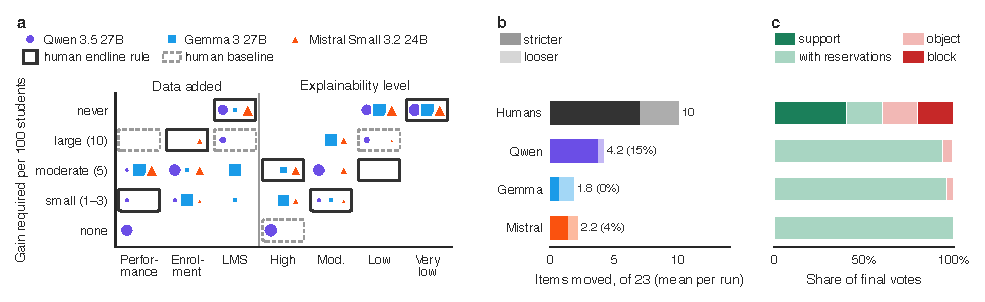
\includegraphics[width=\linewidth]{fig_full.pdf}
  \caption{(a)~Panels' endline answer per rule; marker size = runs (of 20) giving that answer; boxes: human endline (solid), baseline if different (dashed). Rules matched (of 7, mean): Qwen \rulesQwenLargeFull{}, Gemma \rulesGemmaLargeFull{}, Mistral \rulesMistralLargeFull{} (humans' baseline: \humanSelfRules{}); human model chosen: \decisionQwenLargeFull{}, \decisionGemmaLargeFull{}, \decisionMistralLargeFull{} runs. (b)~Items (of 23) whose panel median moved; \% = share of human moves repeated. (c)~Final votes.}
  \label{fig:full}
\end{figure}

\noindent\textbf{What deliberation changed.}
Deliberation changed humans far more than agents (Figure~\ref{fig:full}b).
The humans revised \humanShiftItems{} of 23 answers, mostly toward more restriction, including \humanChangedRules{} of the 7 rules and most sensitive attributes.
Agent panels revised few, rarely in the humans' direction: Qwen also became stricter, but mostly on other items, while Gemma and Mistral mostly loosened sensitive attributes.
Nearly all Gemma and Qwen agents reported becoming more critical.
No agent gave plain support in the final assessment: \reservationsFull{} of votes were ``support with reservations''; humans' ranged from support to block (Figure~\ref{fig:full}c).

\noindent\textbf{Limitations and implications.}
With one workshop, agreement is not validity, but uniform choices, little movement and hedged votes hold regardless and match the ``systematically more cooperative'' simulated users \citet{chen2026trends} warn of, and may manufacture rather than reach consensus \citep[cf.][]{dafoe2020open,tessler2024habermas}. \textbf{Ongoing work} compares deliberation: like humans, agents weighed surveillance against helping students in need and named the harm of being flagged; they dwelt on advisor resources and student wellbeing but did not raise intersectionality or question the system's purpose or its idea of a ``good'' student.

\bibliography{references}

\end{document}
